% documentclass: article used for scientific journals, short reports, program documentation, etc
% options: fontsize 11, generate document for double sided printing, a4-paper
\documentclass[11pt, twoside, a4paper]{article}

% package for changing page layout
\usepackage{geometry}
\geometry{a4paper, lmargin=30mm, rmargin=20mm, tmargin=30mm, bmargin=20mm}
% set indentation
\setlength{\parindent}{0mm} 

% input encoding for special characters (e.g. ä,ü,ö,ß), only for non english text
% options: utf8 as encoding standard
\usepackage[utf8]{inputenc}
% package for changing used language
% options: german or default: english
\usepackage[german]{babel}

% package for math symbols, functions and environments from ams(american mathematical society)
\usepackage{amsmath}
% package for extended symbols from ams
\usepackage{amssymb}
% package for extended symbols from stmaryrd(st mary road)
%\usepackage{stmaryrd}
% package for managing pictures
\usepackage{graphicx}

% package for some extra fonts
\usepackage{txfonts}
% package for changing color of font and paper
% options: using names of default colors (e.g red, black)
\usepackage[usenames]{color}

% package for converting eps-files to pdf-files and then include them
\usepackage{epstopdf}
% use another program (ps2pdf) for converting
% !!! important: set shell_escape=1 in /etc/texmf/texmf.cnf (Linux) for allowing to use other programs
% !!!			 or use the command line with -shell-escape
\epstopdfDeclareGraphicsRule{.eps}{pdf}{.pdf}{
ps2pdf -dEPSCrop #1 \OutputFile
}

% package for reference to last page (output number of last page)
\usepackage{lastpage}
% package for using header and footer
% options: automate terms of right and left marks
\usepackage[automark]{scrpage2}
% set style for footer and header
\pagestyle{scrheadings}
% clear pagestyle for redefining
\clearscrheadfoot
% set header and footer: use <xx>head/foot[]{Text} (i...inner, o...outer, c...center, o...odd, e...even, l...left, r...right)
\ihead[]{}
\ohead[]{}
\cfoot[]{\pagemark/\pageref{LastPage}}


% begin the document
\begin{document}
	
	\begin{figure}
		% GNUPLOT: LaTeX picture with Postscript
\begingroup
  \makeatletter
  \providecommand\color[2][]{%
    \GenericError{(gnuplot) \space\space\space\@spaces}{%
      Package color not loaded in conjunction with
      terminal option `colourtext'%
    }{See the gnuplot documentation for explanation.%
    }{Either use 'blacktext' in gnuplot or load the package
      color.sty in LaTeX.}%
    \renewcommand\color[2][]{}%
  }%
  \providecommand\includegraphics[2][]{%
    \GenericError{(gnuplot) \space\space\space\@spaces}{%
      Package graphicx or graphics not loaded%
    }{See the gnuplot documentation for explanation.%
    }{The gnuplot epslatex terminal needs graphicx.sty or graphics.sty.}%
    \renewcommand\includegraphics[2][]{}%
  }%
  \providecommand\rotatebox[2]{#2}%
  \@ifundefined{ifGPcolor}{%
    \newif\ifGPcolor
    \GPcolorfalse
  }{}%
  \@ifundefined{ifGPblacktext}{%
    \newif\ifGPblacktext
    \GPblacktexttrue
  }{}%
  % define a \g@addto@macro without @ in the name:
  \let\gplgaddtomacro\g@addto@macro
  % define empty templates for all commands taking text:
  \gdef\gplbacktext{}%
  \gdef\gplfronttext{}%
  \makeatother
  \ifGPblacktext
    % no textcolor at all
    \def\colorrgb#1{}%
    \def\colorgray#1{}%
  \else
    % gray or color?
    \ifGPcolor
      \def\colorrgb#1{\color[rgb]{#1}}%
      \def\colorgray#1{\color[gray]{#1}}%
      \expandafter\def\csname LTw\endcsname{\color{white}}%
      \expandafter\def\csname LTb\endcsname{\color{black}}%
      \expandafter\def\csname LTa\endcsname{\color{black}}%
      \expandafter\def\csname LT0\endcsname{\color[rgb]{1,0,0}}%
      \expandafter\def\csname LT1\endcsname{\color[rgb]{0,1,0}}%
      \expandafter\def\csname LT2\endcsname{\color[rgb]{0,0,1}}%
      \expandafter\def\csname LT3\endcsname{\color[rgb]{1,0,1}}%
      \expandafter\def\csname LT4\endcsname{\color[rgb]{0,1,1}}%
      \expandafter\def\csname LT5\endcsname{\color[rgb]{1,1,0}}%
      \expandafter\def\csname LT6\endcsname{\color[rgb]{0,0,0}}%
      \expandafter\def\csname LT7\endcsname{\color[rgb]{1,0.3,0}}%
      \expandafter\def\csname LT8\endcsname{\color[rgb]{0.5,0.5,0.5}}%
    \else
      % gray
      \def\colorrgb#1{\color{black}}%
      \def\colorgray#1{\color[gray]{#1}}%
      \expandafter\def\csname LTw\endcsname{\color{white}}%
      \expandafter\def\csname LTb\endcsname{\color{black}}%
      \expandafter\def\csname LTa\endcsname{\color{black}}%
      \expandafter\def\csname LT0\endcsname{\color{black}}%
      \expandafter\def\csname LT1\endcsname{\color{black}}%
      \expandafter\def\csname LT2\endcsname{\color{black}}%
      \expandafter\def\csname LT3\endcsname{\color{black}}%
      \expandafter\def\csname LT4\endcsname{\color{black}}%
      \expandafter\def\csname LT5\endcsname{\color{black}}%
      \expandafter\def\csname LT6\endcsname{\color{black}}%
      \expandafter\def\csname LT7\endcsname{\color{black}}%
      \expandafter\def\csname LT8\endcsname{\color{black}}%
    \fi
  \fi
  \setlength{\unitlength}{0.0500bp}%
  \begin{picture}(8502.00,6802.00)%
      \csname LTb\endcsname%
      \put(4251,6582){\makebox(0,0){\strut{}Sinusspannung mit $f=100Hz$}}%
    \gplgaddtomacro\gplbacktext{%
      \csname LTb\endcsname%
      \put(946,3995){\makebox(0,0)[r]{\strut{}-0.6}}%
      \put(946,4316){\makebox(0,0)[r]{\strut{}-0.4}}%
      \put(946,4637){\makebox(0,0)[r]{\strut{}-0.2}}%
      \put(946,4958){\makebox(0,0)[r]{\strut{} 0}}%
      \put(946,5279){\makebox(0,0)[r]{\strut{} 0.2}}%
      \put(946,5600){\makebox(0,0)[r]{\strut{} 0.4}}%
      \put(946,5921){\makebox(0,0)[r]{\strut{} 0.6}}%
      \put(1078,3775){\makebox(0,0){\strut{} 0}}%
      \put(2483,3775){\makebox(0,0){\strut{} 0.05}}%
      \put(3889,3775){\makebox(0,0){\strut{} 0.1}}%
      \put(5294,3775){\makebox(0,0){\strut{} 0.15}}%
      \put(6700,3775){\makebox(0,0){\strut{} 0.2}}%
      \put(8105,3775){\makebox(0,0){\strut{} 0.25}}%
      \put(176,4958){\rotatebox{-270}{\makebox(0,0){\strut{}$U \ [V]$}}}%
      \put(4591,3445){\makebox(0,0){\strut{}$t \ [s]$}}%
      \put(4591,6251){\makebox(0,0){\strut{}Zeitverlauf}}%
    }%
    \gplgaddtomacro\gplfronttext{%
    }%
    \gplgaddtomacro\gplbacktext{%
      \csname LTb\endcsname%
      \put(1078,704){\makebox(0,0)[r]{\strut{} 0}}%
      \put(1078,945){\makebox(0,0)[r]{\strut{} 0.05}}%
      \put(1078,1186){\makebox(0,0)[r]{\strut{} 0.1}}%
      \put(1078,1427){\makebox(0,0)[r]{\strut{} 0.15}}%
      \put(1078,1668){\makebox(0,0)[r]{\strut{} 0.2}}%
      \put(1078,1908){\makebox(0,0)[r]{\strut{} 0.25}}%
      \put(1078,2149){\makebox(0,0)[r]{\strut{} 0.3}}%
      \put(1078,2390){\makebox(0,0)[r]{\strut{} 0.35}}%
      \put(1078,2631){\makebox(0,0)[r]{\strut{} 0.4}}%
      \put(1210,484){\makebox(0,0){\strut{} 0}}%
      \put(1900,484){\makebox(0,0){\strut{} 500}}%
      \put(2589,484){\makebox(0,0){\strut{} 1000}}%
      \put(3279,484){\makebox(0,0){\strut{} 1500}}%
      \put(3968,484){\makebox(0,0){\strut{} 2000}}%
      \put(4658,484){\makebox(0,0){\strut{} 2500}}%
      \put(5347,484){\makebox(0,0){\strut{} 3000}}%
      \put(6037,484){\makebox(0,0){\strut{} 3500}}%
      \put(6726,484){\makebox(0,0){\strut{} 4000}}%
      \put(7416,484){\makebox(0,0){\strut{} 4500}}%
      \put(8105,484){\makebox(0,0){\strut{} 5000}}%
      \put(176,1667){\rotatebox{-270}{\makebox(0,0){\strut{}$F$}}}%
      \put(4657,154){\makebox(0,0){\strut{}$f \ [Hz]$}}%
      \put(4657,2961){\makebox(0,0){\strut{}Frequenzspektrum}}%
    }%
    \gplgaddtomacro\gplfronttext{%
    }%
    \gplbacktext
    \put(0,0){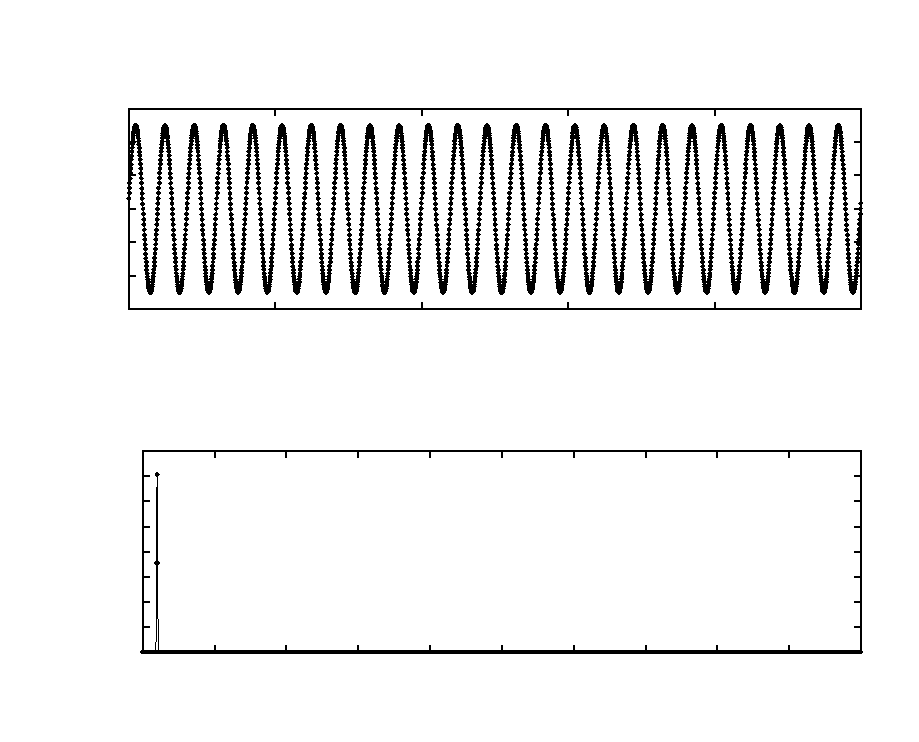
\includegraphics{1-sinus}}%
    \gplfronttext
  \end{picture}%
\endgroup

	\end{figure}

	\begin{figure}
		% GNUPLOT: LaTeX picture with Postscript
\begingroup
  \makeatletter
  \providecommand\color[2][]{%
    \GenericError{(gnuplot) \space\space\space\@spaces}{%
      Package color not loaded in conjunction with
      terminal option `colourtext'%
    }{See the gnuplot documentation for explanation.%
    }{Either use 'blacktext' in gnuplot or load the package
      color.sty in LaTeX.}%
    \renewcommand\color[2][]{}%
  }%
  \providecommand\includegraphics[2][]{%
    \GenericError{(gnuplot) \space\space\space\@spaces}{%
      Package graphicx or graphics not loaded%
    }{See the gnuplot documentation for explanation.%
    }{The gnuplot epslatex terminal needs graphicx.sty or graphics.sty.}%
    \renewcommand\includegraphics[2][]{}%
  }%
  \providecommand\rotatebox[2]{#2}%
  \@ifundefined{ifGPcolor}{%
    \newif\ifGPcolor
    \GPcolorfalse
  }{}%
  \@ifundefined{ifGPblacktext}{%
    \newif\ifGPblacktext
    \GPblacktexttrue
  }{}%
  % define a \g@addto@macro without @ in the name:
  \let\gplgaddtomacro\g@addto@macro
  % define empty templates for all commands taking text:
  \gdef\gplbacktext{}%
  \gdef\gplfronttext{}%
  \makeatother
  \ifGPblacktext
    % no textcolor at all
    \def\colorrgb#1{}%
    \def\colorgray#1{}%
  \else
    % gray or color?
    \ifGPcolor
      \def\colorrgb#1{\color[rgb]{#1}}%
      \def\colorgray#1{\color[gray]{#1}}%
      \expandafter\def\csname LTw\endcsname{\color{white}}%
      \expandafter\def\csname LTb\endcsname{\color{black}}%
      \expandafter\def\csname LTa\endcsname{\color{black}}%
      \expandafter\def\csname LT0\endcsname{\color[rgb]{1,0,0}}%
      \expandafter\def\csname LT1\endcsname{\color[rgb]{0,1,0}}%
      \expandafter\def\csname LT2\endcsname{\color[rgb]{0,0,1}}%
      \expandafter\def\csname LT3\endcsname{\color[rgb]{1,0,1}}%
      \expandafter\def\csname LT4\endcsname{\color[rgb]{0,1,1}}%
      \expandafter\def\csname LT5\endcsname{\color[rgb]{1,1,0}}%
      \expandafter\def\csname LT6\endcsname{\color[rgb]{0,0,0}}%
      \expandafter\def\csname LT7\endcsname{\color[rgb]{1,0.3,0}}%
      \expandafter\def\csname LT8\endcsname{\color[rgb]{0.5,0.5,0.5}}%
    \else
      % gray
      \def\colorrgb#1{\color{black}}%
      \def\colorgray#1{\color[gray]{#1}}%
      \expandafter\def\csname LTw\endcsname{\color{white}}%
      \expandafter\def\csname LTb\endcsname{\color{black}}%
      \expandafter\def\csname LTa\endcsname{\color{black}}%
      \expandafter\def\csname LT0\endcsname{\color{black}}%
      \expandafter\def\csname LT1\endcsname{\color{black}}%
      \expandafter\def\csname LT2\endcsname{\color{black}}%
      \expandafter\def\csname LT3\endcsname{\color{black}}%
      \expandafter\def\csname LT4\endcsname{\color{black}}%
      \expandafter\def\csname LT5\endcsname{\color{black}}%
      \expandafter\def\csname LT6\endcsname{\color{black}}%
      \expandafter\def\csname LT7\endcsname{\color{black}}%
      \expandafter\def\csname LT8\endcsname{\color{black}}%
    \fi
  \fi
  \setlength{\unitlength}{0.0500bp}%
  \begin{picture}(8502.00,6802.00)%
      \csname LTb\endcsname%
      \put(4251,6582){\makebox(0,0){\strut{}Rechteckspannung mit $f=100Hz$}}%
    \gplgaddtomacro\gplbacktext{%
      \csname LTb\endcsname%
      \put(946,3995){\makebox(0,0)[r]{\strut{}-0.6}}%
      \put(946,4316){\makebox(0,0)[r]{\strut{}-0.4}}%
      \put(946,4637){\makebox(0,0)[r]{\strut{}-0.2}}%
      \put(946,4958){\makebox(0,0)[r]{\strut{} 0}}%
      \put(946,5279){\makebox(0,0)[r]{\strut{} 0.2}}%
      \put(946,5600){\makebox(0,0)[r]{\strut{} 0.4}}%
      \put(946,5921){\makebox(0,0)[r]{\strut{} 0.6}}%
      \put(1078,3775){\makebox(0,0){\strut{} 0}}%
      \put(2483,3775){\makebox(0,0){\strut{} 0.05}}%
      \put(3889,3775){\makebox(0,0){\strut{} 0.1}}%
      \put(5294,3775){\makebox(0,0){\strut{} 0.15}}%
      \put(6700,3775){\makebox(0,0){\strut{} 0.2}}%
      \put(8105,3775){\makebox(0,0){\strut{} 0.25}}%
      \put(176,4958){\rotatebox{-270}{\makebox(0,0){\strut{}$U \ [V]$}}}%
      \put(4591,3445){\makebox(0,0){\strut{}$t \ [s]$}}%
      \put(4591,6251){\makebox(0,0){\strut{}Zeitverlauf}}%
    }%
    \gplgaddtomacro\gplfronttext{%
    }%
    \gplgaddtomacro\gplbacktext{%
      \csname LTb\endcsname%
      \put(1078,704){\makebox(0,0)[r]{\strut{} 0}}%
      \put(1078,897){\makebox(0,0)[r]{\strut{} 0.05}}%
      \put(1078,1089){\makebox(0,0)[r]{\strut{} 0.1}}%
      \put(1078,1282){\makebox(0,0)[r]{\strut{} 0.15}}%
      \put(1078,1475){\makebox(0,0)[r]{\strut{} 0.2}}%
      \put(1078,1668){\makebox(0,0)[r]{\strut{} 0.25}}%
      \put(1078,1860){\makebox(0,0)[r]{\strut{} 0.3}}%
      \put(1078,2053){\makebox(0,0)[r]{\strut{} 0.35}}%
      \put(1078,2246){\makebox(0,0)[r]{\strut{} 0.4}}%
      \put(1078,2438){\makebox(0,0)[r]{\strut{} 0.45}}%
      \put(1078,2631){\makebox(0,0)[r]{\strut{} 0.5}}%
      \put(1210,484){\makebox(0,0){\strut{} 0}}%
      \put(1900,484){\makebox(0,0){\strut{} 500}}%
      \put(2589,484){\makebox(0,0){\strut{} 1000}}%
      \put(3279,484){\makebox(0,0){\strut{} 1500}}%
      \put(3968,484){\makebox(0,0){\strut{} 2000}}%
      \put(4658,484){\makebox(0,0){\strut{} 2500}}%
      \put(5347,484){\makebox(0,0){\strut{} 3000}}%
      \put(6037,484){\makebox(0,0){\strut{} 3500}}%
      \put(6726,484){\makebox(0,0){\strut{} 4000}}%
      \put(7416,484){\makebox(0,0){\strut{} 4500}}%
      \put(8105,484){\makebox(0,0){\strut{} 5000}}%
      \put(176,1667){\rotatebox{-270}{\makebox(0,0){\strut{}$F$}}}%
      \put(4657,154){\makebox(0,0){\strut{}$f \ [Hz]$}}%
      \put(4657,2961){\makebox(0,0){\strut{}Frequenzspektrum}}%
    }%
    \gplgaddtomacro\gplfronttext{%
    }%
    \gplbacktext
    \put(0,0){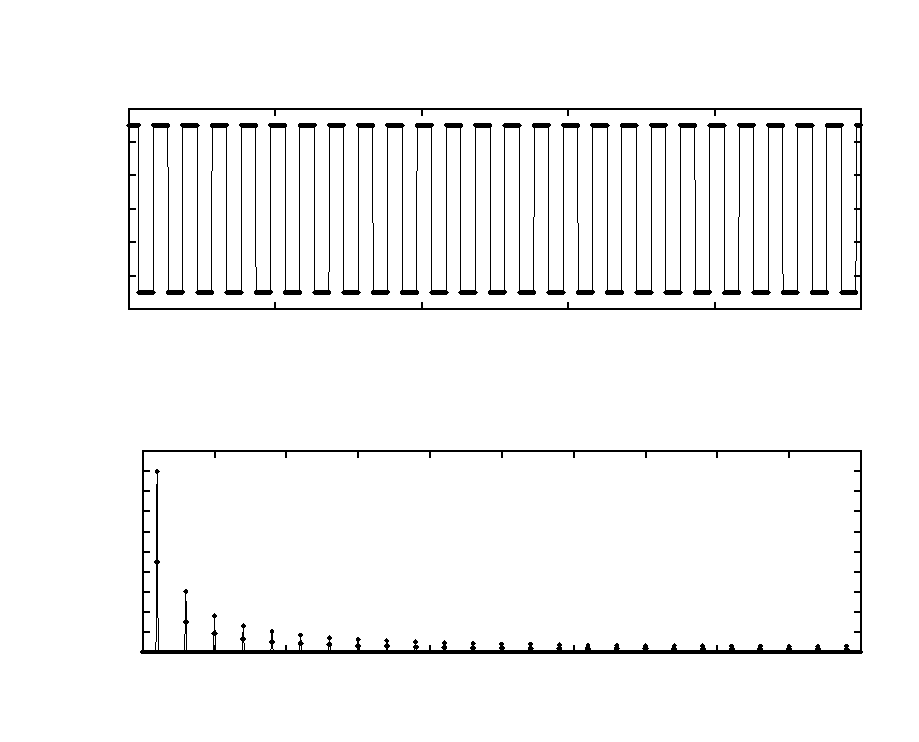
\includegraphics{1-rechteck}}%
    \gplfronttext
  \end{picture}%
\endgroup

	\end{figure}

	\begin{figure}
		% GNUPLOT: LaTeX picture with Postscript
\begingroup
  \makeatletter
  \providecommand\color[2][]{%
    \GenericError{(gnuplot) \space\space\space\@spaces}{%
      Package color not loaded in conjunction with
      terminal option `colourtext'%
    }{See the gnuplot documentation for explanation.%
    }{Either use 'blacktext' in gnuplot or load the package
      color.sty in LaTeX.}%
    \renewcommand\color[2][]{}%
  }%
  \providecommand\includegraphics[2][]{%
    \GenericError{(gnuplot) \space\space\space\@spaces}{%
      Package graphicx or graphics not loaded%
    }{See the gnuplot documentation for explanation.%
    }{The gnuplot epslatex terminal needs graphicx.sty or graphics.sty.}%
    \renewcommand\includegraphics[2][]{}%
  }%
  \providecommand\rotatebox[2]{#2}%
  \@ifundefined{ifGPcolor}{%
    \newif\ifGPcolor
    \GPcolorfalse
  }{}%
  \@ifundefined{ifGPblacktext}{%
    \newif\ifGPblacktext
    \GPblacktexttrue
  }{}%
  % define a \g@addto@macro without @ in the name:
  \let\gplgaddtomacro\g@addto@macro
  % define empty templates for all commands taking text:
  \gdef\gplbacktext{}%
  \gdef\gplfronttext{}%
  \makeatother
  \ifGPblacktext
    % no textcolor at all
    \def\colorrgb#1{}%
    \def\colorgray#1{}%
  \else
    % gray or color?
    \ifGPcolor
      \def\colorrgb#1{\color[rgb]{#1}}%
      \def\colorgray#1{\color[gray]{#1}}%
      \expandafter\def\csname LTw\endcsname{\color{white}}%
      \expandafter\def\csname LTb\endcsname{\color{black}}%
      \expandafter\def\csname LTa\endcsname{\color{black}}%
      \expandafter\def\csname LT0\endcsname{\color[rgb]{1,0,0}}%
      \expandafter\def\csname LT1\endcsname{\color[rgb]{0,1,0}}%
      \expandafter\def\csname LT2\endcsname{\color[rgb]{0,0,1}}%
      \expandafter\def\csname LT3\endcsname{\color[rgb]{1,0,1}}%
      \expandafter\def\csname LT4\endcsname{\color[rgb]{0,1,1}}%
      \expandafter\def\csname LT5\endcsname{\color[rgb]{1,1,0}}%
      \expandafter\def\csname LT6\endcsname{\color[rgb]{0,0,0}}%
      \expandafter\def\csname LT7\endcsname{\color[rgb]{1,0.3,0}}%
      \expandafter\def\csname LT8\endcsname{\color[rgb]{0.5,0.5,0.5}}%
    \else
      % gray
      \def\colorrgb#1{\color{black}}%
      \def\colorgray#1{\color[gray]{#1}}%
      \expandafter\def\csname LTw\endcsname{\color{white}}%
      \expandafter\def\csname LTb\endcsname{\color{black}}%
      \expandafter\def\csname LTa\endcsname{\color{black}}%
      \expandafter\def\csname LT0\endcsname{\color{black}}%
      \expandafter\def\csname LT1\endcsname{\color{black}}%
      \expandafter\def\csname LT2\endcsname{\color{black}}%
      \expandafter\def\csname LT3\endcsname{\color{black}}%
      \expandafter\def\csname LT4\endcsname{\color{black}}%
      \expandafter\def\csname LT5\endcsname{\color{black}}%
      \expandafter\def\csname LT6\endcsname{\color{black}}%
      \expandafter\def\csname LT7\endcsname{\color{black}}%
      \expandafter\def\csname LT8\endcsname{\color{black}}%
    \fi
  \fi
  \setlength{\unitlength}{0.0500bp}%
  \begin{picture}(8502.00,6802.00)%
      \csname LTb\endcsname%
      \put(4251,6582){\makebox(0,0){\strut{}Dreieckspannung mit $f=100Hz$}}%
    \gplgaddtomacro\gplbacktext{%
      \csname LTb\endcsname%
      \put(946,3995){\makebox(0,0)[r]{\strut{}-0.5}}%
      \put(946,4188){\makebox(0,0)[r]{\strut{}-0.4}}%
      \put(946,4380){\makebox(0,0)[r]{\strut{}-0.3}}%
      \put(946,4573){\makebox(0,0)[r]{\strut{}-0.2}}%
      \put(946,4765){\makebox(0,0)[r]{\strut{}-0.1}}%
      \put(946,4958){\makebox(0,0)[r]{\strut{} 0}}%
      \put(946,5151){\makebox(0,0)[r]{\strut{} 0.1}}%
      \put(946,5343){\makebox(0,0)[r]{\strut{} 0.2}}%
      \put(946,5536){\makebox(0,0)[r]{\strut{} 0.3}}%
      \put(946,5728){\makebox(0,0)[r]{\strut{} 0.4}}%
      \put(946,5921){\makebox(0,0)[r]{\strut{} 0.5}}%
      \put(1078,3775){\makebox(0,0){\strut{} 0}}%
      \put(2483,3775){\makebox(0,0){\strut{} 0.05}}%
      \put(3889,3775){\makebox(0,0){\strut{} 0.1}}%
      \put(5294,3775){\makebox(0,0){\strut{} 0.15}}%
      \put(6700,3775){\makebox(0,0){\strut{} 0.2}}%
      \put(8105,3775){\makebox(0,0){\strut{} 0.25}}%
      \put(176,4958){\rotatebox{-270}{\makebox(0,0){\strut{}$U \ [V]$}}}%
      \put(4591,3445){\makebox(0,0){\strut{}$t \ [s]$}}%
      \put(4591,6251){\makebox(0,0){\strut{}Zeitverlauf}}%
    }%
    \gplgaddtomacro\gplfronttext{%
    }%
    \gplgaddtomacro\gplbacktext{%
      \csname LTb\endcsname%
      \put(1078,704){\makebox(0,0)[r]{\strut{} 0}}%
      \put(1078,1025){\makebox(0,0)[r]{\strut{} 0.05}}%
      \put(1078,1346){\makebox(0,0)[r]{\strut{} 0.1}}%
      \put(1078,1668){\makebox(0,0)[r]{\strut{} 0.15}}%
      \put(1078,1989){\makebox(0,0)[r]{\strut{} 0.2}}%
      \put(1078,2310){\makebox(0,0)[r]{\strut{} 0.25}}%
      \put(1078,2631){\makebox(0,0)[r]{\strut{} 0.3}}%
      \put(1210,484){\makebox(0,0){\strut{} 0}}%
      \put(1900,484){\makebox(0,0){\strut{} 500}}%
      \put(2589,484){\makebox(0,0){\strut{} 1000}}%
      \put(3279,484){\makebox(0,0){\strut{} 1500}}%
      \put(3968,484){\makebox(0,0){\strut{} 2000}}%
      \put(4658,484){\makebox(0,0){\strut{} 2500}}%
      \put(5347,484){\makebox(0,0){\strut{} 3000}}%
      \put(6037,484){\makebox(0,0){\strut{} 3500}}%
      \put(6726,484){\makebox(0,0){\strut{} 4000}}%
      \put(7416,484){\makebox(0,0){\strut{} 4500}}%
      \put(8105,484){\makebox(0,0){\strut{} 5000}}%
      \put(176,1667){\rotatebox{-270}{\makebox(0,0){\strut{}$F$}}}%
      \put(4657,154){\makebox(0,0){\strut{}$f \ [Hz]$}}%
      \put(4657,2961){\makebox(0,0){\strut{}Frequenzspektrum}}%
    }%
    \gplgaddtomacro\gplfronttext{%
    }%
    \gplbacktext
    \put(0,0){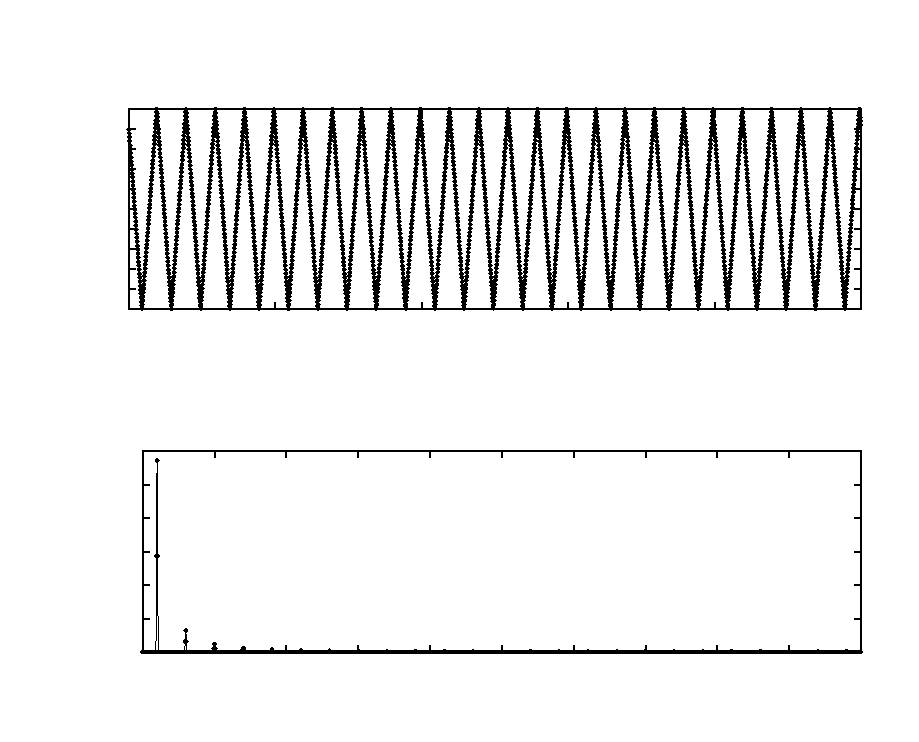
\includegraphics{1-dreieck}}%
    \gplfronttext
  \end{picture}%
\endgroup

	\end{figure}

	\begin{figure}
		% GNUPLOT: LaTeX picture with Postscript
\begingroup
  \makeatletter
  \providecommand\color[2][]{%
    \GenericError{(gnuplot) \space\space\space\@spaces}{%
      Package color not loaded in conjunction with
      terminal option `colourtext'%
    }{See the gnuplot documentation for explanation.%
    }{Either use 'blacktext' in gnuplot or load the package
      color.sty in LaTeX.}%
    \renewcommand\color[2][]{}%
  }%
  \providecommand\includegraphics[2][]{%
    \GenericError{(gnuplot) \space\space\space\@spaces}{%
      Package graphicx or graphics not loaded%
    }{See the gnuplot documentation for explanation.%
    }{The gnuplot epslatex terminal needs graphicx.sty or graphics.sty.}%
    \renewcommand\includegraphics[2][]{}%
  }%
  \providecommand\rotatebox[2]{#2}%
  \@ifundefined{ifGPcolor}{%
    \newif\ifGPcolor
    \GPcolorfalse
  }{}%
  \@ifundefined{ifGPblacktext}{%
    \newif\ifGPblacktext
    \GPblacktexttrue
  }{}%
  % define a \g@addto@macro without @ in the name:
  \let\gplgaddtomacro\g@addto@macro
  % define empty templates for all commands taking text:
  \gdef\gplbacktext{}%
  \gdef\gplfronttext{}%
  \makeatother
  \ifGPblacktext
    % no textcolor at all
    \def\colorrgb#1{}%
    \def\colorgray#1{}%
  \else
    % gray or color?
    \ifGPcolor
      \def\colorrgb#1{\color[rgb]{#1}}%
      \def\colorgray#1{\color[gray]{#1}}%
      \expandafter\def\csname LTw\endcsname{\color{white}}%
      \expandafter\def\csname LTb\endcsname{\color{black}}%
      \expandafter\def\csname LTa\endcsname{\color{black}}%
      \expandafter\def\csname LT0\endcsname{\color[rgb]{1,0,0}}%
      \expandafter\def\csname LT1\endcsname{\color[rgb]{0,1,0}}%
      \expandafter\def\csname LT2\endcsname{\color[rgb]{0,0,1}}%
      \expandafter\def\csname LT3\endcsname{\color[rgb]{1,0,1}}%
      \expandafter\def\csname LT4\endcsname{\color[rgb]{0,1,1}}%
      \expandafter\def\csname LT5\endcsname{\color[rgb]{1,1,0}}%
      \expandafter\def\csname LT6\endcsname{\color[rgb]{0,0,0}}%
      \expandafter\def\csname LT7\endcsname{\color[rgb]{1,0.3,0}}%
      \expandafter\def\csname LT8\endcsname{\color[rgb]{0.5,0.5,0.5}}%
    \else
      % gray
      \def\colorrgb#1{\color{black}}%
      \def\colorgray#1{\color[gray]{#1}}%
      \expandafter\def\csname LTw\endcsname{\color{white}}%
      \expandafter\def\csname LTb\endcsname{\color{black}}%
      \expandafter\def\csname LTa\endcsname{\color{black}}%
      \expandafter\def\csname LT0\endcsname{\color{black}}%
      \expandafter\def\csname LT1\endcsname{\color{black}}%
      \expandafter\def\csname LT2\endcsname{\color{black}}%
      \expandafter\def\csname LT3\endcsname{\color{black}}%
      \expandafter\def\csname LT4\endcsname{\color{black}}%
      \expandafter\def\csname LT5\endcsname{\color{black}}%
      \expandafter\def\csname LT6\endcsname{\color{black}}%
      \expandafter\def\csname LT7\endcsname{\color{black}}%
      \expandafter\def\csname LT8\endcsname{\color{black}}%
    \fi
  \fi
  \setlength{\unitlength}{0.0500bp}%
  \begin{picture}(8502.00,6802.00)%
      \csname LTb\endcsname%
      \put(4251,6582){\makebox(0,0){\strut{}Rauschspannung}}%
    \gplgaddtomacro\gplbacktext{%
      \csname LTb\endcsname%
      \put(1078,3995){\makebox(0,0)[r]{\strut{}-0.15}}%
      \put(1078,4316){\makebox(0,0)[r]{\strut{}-0.1}}%
      \put(1078,4637){\makebox(0,0)[r]{\strut{}-0.05}}%
      \put(1078,4958){\makebox(0,0)[r]{\strut{} 0}}%
      \put(1078,5279){\makebox(0,0)[r]{\strut{} 0.05}}%
      \put(1078,5600){\makebox(0,0)[r]{\strut{} 0.1}}%
      \put(1078,5921){\makebox(0,0)[r]{\strut{} 0.15}}%
      \put(1210,3775){\makebox(0,0){\strut{} 0}}%
      \put(2589,3775){\makebox(0,0){\strut{} 0.05}}%
      \put(3968,3775){\makebox(0,0){\strut{} 0.1}}%
      \put(5347,3775){\makebox(0,0){\strut{} 0.15}}%
      \put(6726,3775){\makebox(0,0){\strut{} 0.2}}%
      \put(8105,3775){\makebox(0,0){\strut{} 0.25}}%
      \put(176,4958){\rotatebox{-270}{\makebox(0,0){\strut{}$U \ [V]$}}}%
      \put(4657,3445){\makebox(0,0){\strut{}$t \ [s]$}}%
      \put(4657,6251){\makebox(0,0){\strut{}Zeitverlauf}}%
    }%
    \gplgaddtomacro\gplfronttext{%
    }%
    \gplgaddtomacro\gplbacktext{%
      \csname LTb\endcsname%
      \put(1210,704){\makebox(0,0)[r]{\strut{} 0}}%
      \put(1210,979){\makebox(0,0)[r]{\strut{} 0.001}}%
      \put(1210,1255){\makebox(0,0)[r]{\strut{} 0.002}}%
      \put(1210,1530){\makebox(0,0)[r]{\strut{} 0.003}}%
      \put(1210,1805){\makebox(0,0)[r]{\strut{} 0.004}}%
      \put(1210,2080){\makebox(0,0)[r]{\strut{} 0.005}}%
      \put(1210,2356){\makebox(0,0)[r]{\strut{} 0.006}}%
      \put(1210,2631){\makebox(0,0)[r]{\strut{} 0.007}}%
      \put(1342,484){\makebox(0,0){\strut{} 0}}%
      \put(2018,484){\makebox(0,0){\strut{} 500}}%
      \put(2695,484){\makebox(0,0){\strut{} 1000}}%
      \put(3371,484){\makebox(0,0){\strut{} 1500}}%
      \put(4047,484){\makebox(0,0){\strut{} 2000}}%
      \put(4724,484){\makebox(0,0){\strut{} 2500}}%
      \put(5400,484){\makebox(0,0){\strut{} 3000}}%
      \put(6076,484){\makebox(0,0){\strut{} 3500}}%
      \put(6752,484){\makebox(0,0){\strut{} 4000}}%
      \put(7429,484){\makebox(0,0){\strut{} 4500}}%
      \put(8105,484){\makebox(0,0){\strut{} 5000}}%
      \put(176,1667){\rotatebox{-270}{\makebox(0,0){\strut{}$F$}}}%
      \put(4723,154){\makebox(0,0){\strut{}$f \ [Hz]$}}%
      \put(4723,2961){\makebox(0,0){\strut{}Frequenzspektrum}}%
    }%
    \gplgaddtomacro\gplfronttext{%
    }%
    \gplbacktext
    \put(0,0){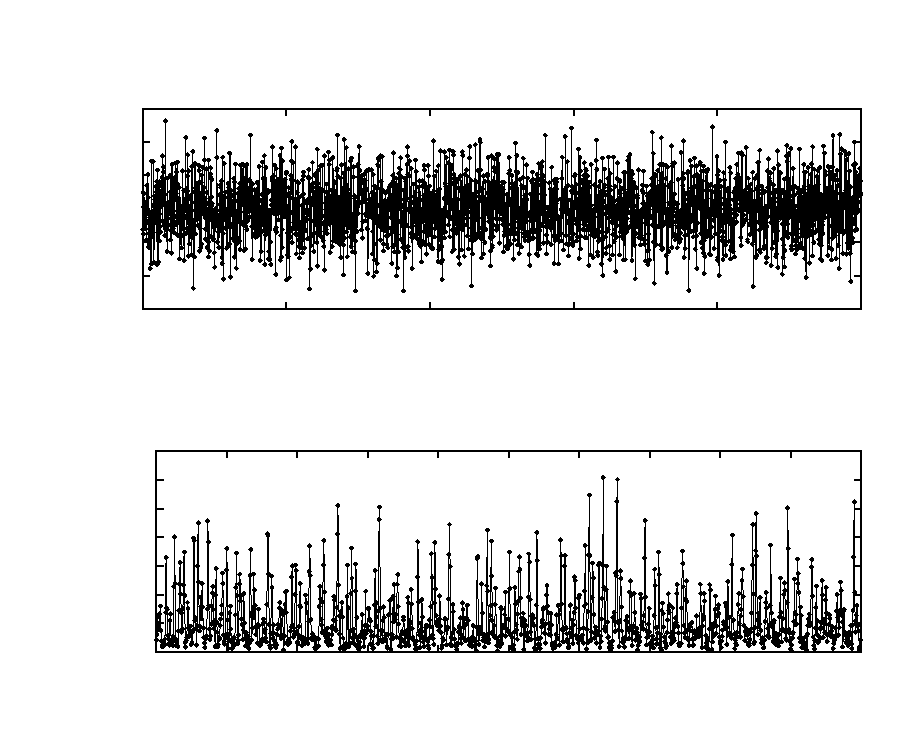
\includegraphics{1-noise}}%
    \gplfronttext
  \end{picture}%
\endgroup

	\end{figure}

\end{document}

